\documentclass[10pt]{standalone}
\usepackage[sc]{mathpazo}
\usepackage{commands}
\renewcommand{\phi}{\varphi}

\begin{document}
\centering
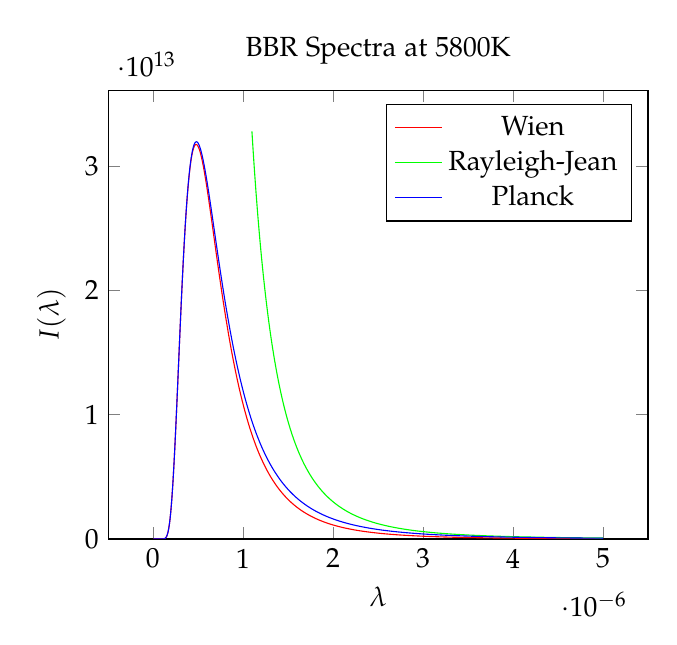
\begin{tikzpicture}
    \begin{axis}[xlabel = $\lambda$, ylabel = $I(\lambda)$, title = BBR Spectra at 5800K, legend pos = north east, ymin = 0]
    \addplot [domain=0:0.000005, samples=1000, color=red]{1.2*10^(-16)/x^5*exp(-2.4*10^(-6)/x)};
    \addplot [domain=0.0000011:0.000005, samples=1000, color=green]{4.8*10^(-11)/x^4};
    \addplot [domain=0:0.000005, samples=1000, color=blue]{1.2*10^(-16)/x^5 /(exp(2.4*10^(-6)/x)-1)};
    \legend{Wien, Rayleigh-Jean, Planck}
    \end{axis}
\end{tikzpicture}
\end{document}